\documentclass[dvipdfmx]{article}
\usepackage[dvipdfmx]{graphicx}
\usepackage{amsmath, amssymb}
\usepackage{mathtools}
\usepackage{here}
\begin{document}
\title{Weekly Report}
\author{Riku Gondow}
\maketitle
\section{Progress}
\begin{itemize}
    \item Check accuracy in Keio Hospital Dataset
    \item Implement EMD(Empirical Mode Decomposition), EEMD(Ensemble Empirical Mode Decomposition)
    \item Receive radar data from Ishizaka-San's Server
\end{itemize}

\subsection*{Identification in Keio Hospital Dataset}

\begin{table}[H]
\caption{Hyper parameter}
\centering
\begin{tabular}{c|c}
\hline
the number of Class & 12 \\
batch size & 64 \\
learning rate & 0.001 \\
epoch & 100 \\
window & 5 s \\
overlap & 1.5 s \\
alpha (center loss) & 0.1\\
\hline
\end{tabular}
\end{table}

\begin{table}[H]
\caption{Accuracy when only BPF is applied}
\centering
\begin{tabular}{c||c}
\hline
CrossEntropy Loss & 45.69 \% \\
Softmax Loss + Center Loss & 47.27 \% \\
Triple Joint Loss(Softmax + Center + Cosine Loss) & 4.23 \% \\
\hline
\end{tabular}
\end{table}

Calculations are currently underway for data with EMD and EEMD applied.

\begin{figure}[htbp]
    \begin{minipage}[c]{0.5\hsize}
      \centering
      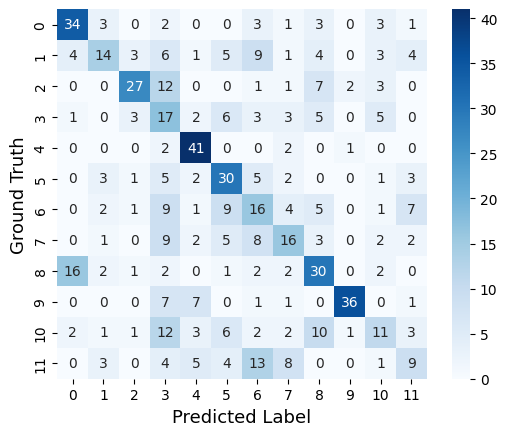
\includegraphics[width=\linewidth]{./img/conf_crossentropy.png}
      \caption{Confusion Matrix with CrossEntropyLoss}
    %   \label{fig:statue}
    \end{minipage}
    \begin{minipage}[c]{0.5\hsize}
      \centering
      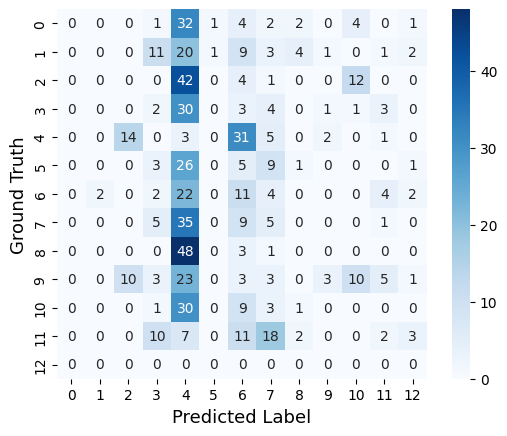
\includegraphics[width=\linewidth]{./img/conf_TJL.png}
      \caption{Confusion Matrix with TripleJointLoss}
    %   \label{fig:spaceship}
    \end{minipage}
  \end{figure}

\subsection*{Application of EMD and EEMD to the data}
\begin{figure}[H]
\begin{center}
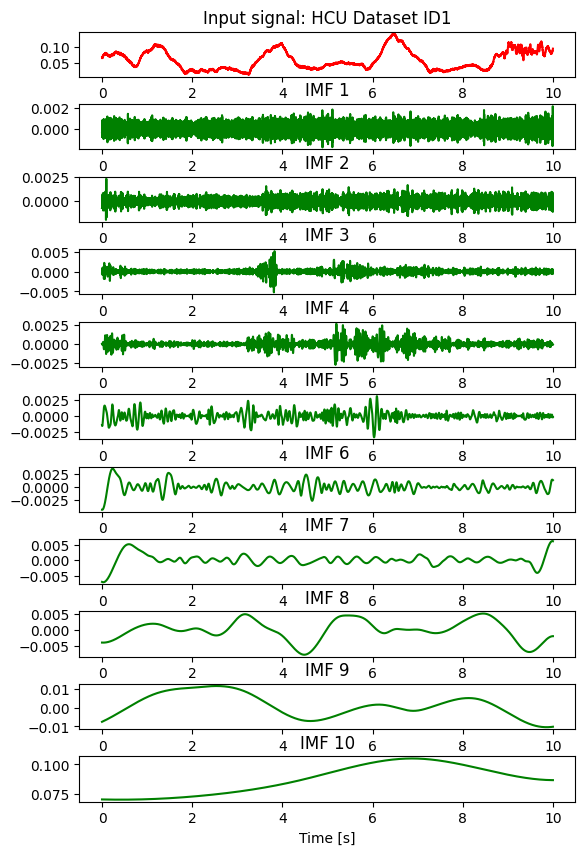
\includegraphics[width=0.8\linewidth]{./img/EMD.png}
\end{center}
\caption{Application of EMD to ID1}
\end{figure}

\begin{figure}[H]
\begin{center}
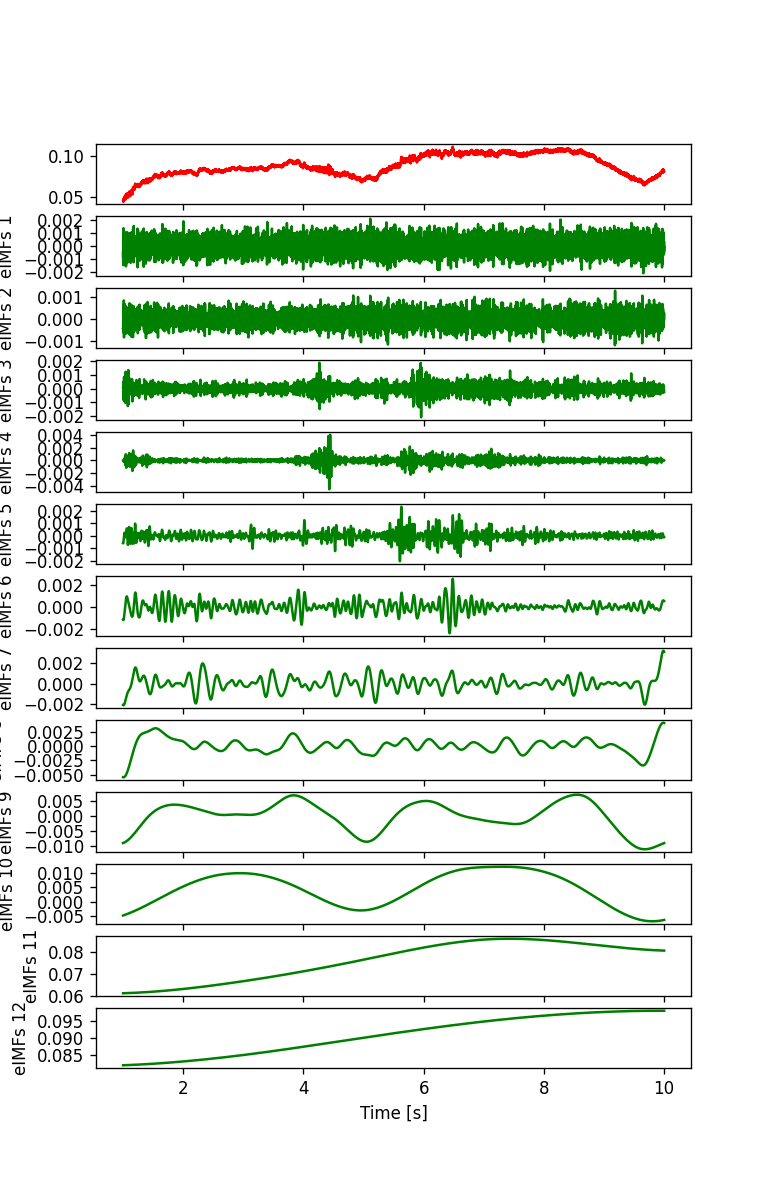
\includegraphics[width=0.9\linewidth]{./img/eemd_example.png}
\end{center}
\caption{Application of EEMD to ID1}
\end{figure}

\section{Next Plan}
\begin{itemize}
    \item Improve the methods for Identification in Keio Hospital Dataset((e.g., adjust hyperparameter, change the classifier to openmax, adopt a denoising method other than BPF, etc.))
\end{itemize}
\end{document}